\chapter{Wyniki testów}
Wyniki testów każdej aplikacji uruchamianej w poszczególnych przypadkach  testowych przedstawiono w formie diagramów: diagramu przedstawiającego liczbę żądań obsłużonych przez aplikację w ciągu sekundy i diagramu rozkładu czasów odpowiedzi aplikacji.

Wyniki testów podzielono na dwie grupy zależne  od początkowego stanu bazy danych.

\section{Testy z pustą bazą danych}

\subsection{Test wydajności walidacji API}
Wyniki testów wydajności walidujących istnienie klucza API przedstawiają diagramy zamieszczone na rysunkach \ref{fig:tomcat_clean_api_validation_rps} - \ref{fig:go_clean_api_validation_td}.

Z diagramów prezentujących liczbę żądań obsłużonych w ciągu sekundy przez poszczególne aplikacje (rys. \ref{fig:tomcat_clean_api_validation_rps}, \ref{fig:jetty_clean_api_validation_rps}, \ref{fig:go_clean_api_validation_rps}) wynika, że przy 100 klientach największą liczbę żądań obsłużyła aplikacja napisana w \textsl{Go} - od 9.0 do 11.0 tysięcy obsłużonych żądań. Wydajność serwera \textsl{Jetty} oscylowała w przedziale od 5.0 do 10.0 tysięcy obsłużonych żądań, przy znacznych wahaniach przepustowości. Przepustowość serwera \textsl{Tomcat} oscylowała w przedziale od 6.0 do 8.0 tysięcy obsłużonych żądań. Przy 250 klientach wydajność aplikacji w \textsl{Go} oscylowała w przedziale od 8.0 do 10.0 tysięcy obsłużonych żądań, a serwery \textsl{Jetty} i \textsl{Tomcat} obsłużyły od 4.0 do 8.0 tysięcy żądań przy dużych wahaniach przepustowości.      

Z diagramów rozkładu czasów odpowiedzi aplikacji (rys. \ref{fig:tomcat_clean_api_validation_td}, \ref{fig:jetty_clean_api_validation_td}, \ref{fig:go_clean_api_validation_td}) wynika, że przy 100 klientach średnie czasy odpowiedzi wynosiły: dla serwera \textsl{Tomcat} 13.70 milisekund, dla serwera \textsl{Jetty} 11.42 milisekund, a dla aplikacji w \textsl{Go} 9,44 milisekundy. Najdłużej trwające żądania trwały około 35 milisekund w przypadku serwerów \textsl{Tomcat} i \textsl{Jetty} oraz 18 milisekund przy aplikacji w \textsl{Go}. Przy 250 klientach średnie czasy odpowiedzi aplikacji uruchamianych na serwerach \textsl{Tomcat} i \textsl{Jetty} były prawie takie same i wynosiły odpowiednio 36.32 i 35.52 milisekund, a w aplikacji w \textsl{Go} 22t.47 milisekundy. Najdłużej trwające żądania trwały ponad 90 milisekund w przypadku serwera Tomcat, poniżej 88 milisekund w przypadku serwera \textsl{Jetty} i około 55 milisekundy przy aplikacji w \textsl{Go}. Dodatkowo, przy 250 klientach, dla serwerów \textsl{Tomcat} i \textsl{Jetty} rozkłady czasów odpowiedzi były spłaszczone. 

\pgfplotsset{grid style={dashed}}
\begin{figure}[!ht]
\pgfplotstableread[col sep = comma]{csv_queries/requests_per_sec/tomcat_clean_api_validation.csv}\csvdata
\begin{tikzpicture}
  \begin{axis}[xmin = 0, xmax=900, ymin = 0, scaled y ticks = base 10:-3, xlabel = {Czas [s]}, ylabel = Liczba żądań, legend pos=south east, ymajorgrids,width=13cm, height=6cm] %TODO miary?
    \addplot[color=blue,mark=none] table[x index=0, y index=1]{\csvdata};
    \addplot[color=green,mark=none] table[x index=0, y index=2]{\csvdata};
    \legend{100 klientów,250 klientów}
  \end{axis}
\end{tikzpicture}
\caption{Tomcat 8 - liczba żądań obsłużonych przez aplikację w ciągu sekundy podczas testu walidacji istnienia klucza API}
\label{fig:tomcat_clean_api_validation_rps}
\end{figure}

\begin{figure}[!ht]
\pgfplotstableread[col sep = comma]{csv_queries/response_time_distribution/tomcat_clean_api_validation_100.csv}\csva
\pgfplotstableread[col sep = comma]{csv_queries/response_time_distribution/tomcat_clean_api_validation_250.csv}\csvb
\pgfplotsset{
    /pgfplots/ybar legend/.style={
    /pgfplots/legend image code/.code={\draw[##1,/tikz/.cd,yshift=-0.25em](0cm,0cm) rectangle(1pt,0.7em);},
   }
}
\begin{tikzpicture}
  \begin{axis}[ybar, bar width=0.5, xmin = 0, ymin = 0, scaled y ticks = base 10:-5, xlabel = {Czas odpowiedzi [ms]}, ylabel = {Liczba żądań}, ymajorgrids,width=13cm, height=6cm] %TODO miary?
    \addplot[color=blue, mark=none, fill=blue] table[x index=0, y index=1]{\csva};
    \addplot[color=green, mark=none, fill=green] table[x index=0, y index=1]{\csvb};
    \legend{100 klientów,250 klientów}
  \end{axis}
\end{tikzpicture}
\caption{Tomcat 8 - rozkład czasów odpowiedzi aplikacji (95\% odpowiedzi) podczas testu walidacji istnienia klucza API}
\label{fig:tomcat_clean_api_validation_td}
\end{figure}

\pgfplotsset{grid style={dashed}}
\begin{figure}[!ht]
\pgfplotstableread[col sep = comma]{csv_queries/requests_per_sec/jetty_clean_api_validation.csv}\csvdata
\begin{tikzpicture}
  \begin{axis}[xmin = 0, xmax=900, ymin = 0, scaled y ticks = base 10:-3, xlabel = {Czas [s]}, ylabel = Liczba żądań, legend pos=south east, ymajorgrids,width=13cm, height=6cm] %TODO miary?
    \addplot[color=blue,mark=none] table[x index=0, y index=1]{\csvdata};
    \addplot[color=green,mark=none] table[x index=0, y index=2]{\csvdata};
    \legend{100 klientów,250 klientów}
  \end{axis}
\end{tikzpicture}
\caption{Jetty 9 - liczba żądań obsłużonych przez aplikację w ciągu sekundy podczas testu walidacji istnienia klucza API}
\label{fig:jetty_clean_api_validation_rps}
\end{figure}

\begin{figure}[!ht]
\pgfplotstableread[col sep = comma]{csv_queries/response_time_distribution/jetty_clean_api_validation_100.csv}\csva
\pgfplotstableread[col sep = comma]{csv_queries/response_time_distribution/jetty_clean_api_validation_250.csv}\csvb
\pgfplotsset{
    /pgfplots/ybar legend/.style={
    /pgfplots/legend image code/.code={\draw[##1,/tikz/.cd,yshift=-0.25em](0cm,0cm) rectangle(1pt,0.7em);},
   }
}
\begin{tikzpicture}
  \begin{axis}[ybar, bar width=0.5, xmin = 0, ymin = 0, scaled y ticks = base 10:-5, xlabel = {Czas odpowiedzi [ms]}, ylabel = {Liczba żądań}, ymajorgrids,width=13cm, height=6cm] %TODO miary?
    \addplot[color=blue, mark=none, fill=blue] table[x index=0, y index=1]{\csva};
    \addplot[color=green, mark=none, fill=green] table[x index=0, y index=1]{\csvb};
    \legend{100 klientów,250 klientów}
  \end{axis}
\end{tikzpicture}
\caption{Jetty 9 - rozkład czasów odpowiedzi aplikacji (95\% odpowiedzi) podczas testu walidacji istnienia klucza API}
\label{fig:jetty_clean_api_validation_td}
\end{figure}

\pgfplotsset{grid style={dashed}}
\begin{figure}[!ht]
\pgfplotstableread[col sep = comma]{csv_queries/requests_per_sec/go_clean_api_validation.csv}\csvdata
\begin{tikzpicture}
  \begin{axis}[xmin = 0, xmax=900, ymin = 0, scaled y ticks = base 10:-3, xlabel = {Czas [s]}, ylabel = Liczba żądań, legend pos=south east, ymajorgrids,width=13cm, height=6cm] %TODO miary?
    \addplot[color=blue,mark=none] table[x index=0, y index=1]{\csvdata};
    \addplot[color=green,mark=none] table[x index=0, y index=2]{\csvdata};
    \legend{100 klientów,250 klientów}
  \end{axis}
\end{tikzpicture}
\caption{Go - liczba żądań obsłużonych przez aplikację w ciągu sekundy podczas testu walidacji istnienia klucza API}
\label{fig:go_clean_api_validation_rps}
\end{figure}

\begin{figure}[!ht]
\pgfplotstableread[col sep = comma]{csv_queries/response_time_distribution/go_clean_api_validation_100.csv}\csva
\pgfplotstableread[col sep = comma]{csv_queries/response_time_distribution/go_clean_api_validation_250.csv}\csvb
\pgfplotsset{
    /pgfplots/ybar legend/.style={
    /pgfplots/legend image code/.code={\draw[##1,/tikz/.cd,yshift=-0.25em](0cm,0cm) rectangle(1pt,0.7em);},
   }
}
\begin{tikzpicture}
  \begin{axis}[ybar, bar width=0.5, xmin = 0, ymin = 0, scaled y ticks = base 10:-5, xlabel = {Czas odpowiedzi [ms]}, ylabel = {Liczba żądań}, ymajorgrids,width=13cm, height=6cm] %TODO miary?
    \addplot[color=blue, mark=none, fill=blue] table[x index=0, y index=1]{\csva};
    \addplot[color=green, mark=none, fill=green] table[x index=0, y index=1]{\csvb};
    \legend{100 klientów,250 klientów}
  \end{axis}
\end{tikzpicture}
\caption{Go - rozkład czasów odpowiedzi aplikacji (95\% odpowiedzi) podczas testu walidacji istnienia klucza API}
\label{fig:go_clean_api_validation_td}
\end{figure}


\clearpage

\subsection{Test wydajności walidacji istnienia obiektów Cache}
Wyniki testów wydajności walidacji istnienia obiektów Cache przedstawiają diagramy na rysunkach \ref{fig:tomcat_clean_key_validation_rps} - \ref{fig:go_clean_key_validation_td}.              

Z diagramów przedstawiających rozkład ilości żądań obsłużonych przez poszczególne aplikacje w ciągu sekundy  (rys. \ref{fig:tomcat_clean_key_validation_rps} \ref{fig:jetty_clean_key_validation_rps}, \ref{fig:go_clean_key_validation_rps}) wynika, że przy 100 klientach największą liczbę żądań (około 7.0 tysięcy) obsłużyła aplikacja napisana w \textsl{Go}. Wydajność serwera \textsl{Jetty} oscylowała w przedziale od 3.5 do 4.5 tysiąca obsłużonych żądań, a serwera \textsl{Tomcat} w przedziale od 2.0 do 3.5 tysiąca obsłużonych żądań. Przy 250 klientach wydajność aplikacji w \textsl{Go} oscylowała w przedziale od 7.0 do 8.0 tysięcy obsłużonych żądań, serwer \textsl{Jetty} obsłużył około 3.0 tysięcy żądań, a serwer \textsl{Tomcat} od 2.0 do 3.5 tysiąca żądań.

Z diagramów rozkładu czasów odpowiedzi (rys. \ref{fig:tomcat_clean_key_validation_td}, \ref{fig:jetty_clean_key_validation_td}, \ref{fig:go_clean_key_validation_td}) wynika, że przy 100 klientach średnie czasy odpowiedzi wynosiły: dla serwera \textsl{Tomcat} 30.32 milisekund, dla serwera \textsl{Jetty} 23.32 milisekund, a dla aplikacji w \textsl{Go} 13.79 milisekund. Najdłużej trwające żądania trwały około 120 milisekund w przypadku serwera Tomcat, 45 milisekund przy \textsl{Jetty} i tylko 25 milisekund w aplikacji w \textsl{Go}. Przy 250 klientach średnie czasy odpowiedzi aplikacji uruchamianych na serwerach \textsl{Tomcat} i \textsl{Jetty} wynosiły odpowiednio 69.97 i 76.92 milisekundy, a w aplikacji w \textsl{Go} tylko 30.75 milisekundy. Najdłużej trwające żądania trwały 250 milisekund w przypadku serwera Tomcat, okło 120 milisekund w przypadku serwera \textsl{Jetty} i tylko 65 milisekundy przy aplikacji w \textsl{Go}. Czasy odpowiedzi serwera \textsl{Tomcat} w sporej części o były dużo dłuższe niż pokazuje to średnia.

\pgfplotsset{grid style={dashed}}
\begin{figure}[!ht]
\pgfplotstableread[col sep = comma]{csv_queries/requests_per_sec/tomcat_clean_key_validation.csv}\csvdata
\begin{tikzpicture}
  \begin{axis}[xmin = 0, xmax=900, ymin = 0, scaled y ticks = base 10:-3, xlabel = {Czas [s]}, ylabel = Liczba żądań, legend pos=south east, ymajorgrids,width=13cm, height=6cm] %TODO miary?
    \addplot[color=blue,mark=none] table[x index=0, y index=1]{\csvdata};
    \addplot[color=green,mark=none] table[x index=0, y index=2]{\csvdata};
    \legend{100 klientów,250 klientów}
  \end{axis}
\end{tikzpicture}
\caption{Tomcat 8 - liczba żądań obsłużonych przez aplikację w ciągu sekundy podczas testu walidacji istnienia rekordu w bazie}
\label{fig:tomcat_clean_key_validation_rps}
\end{figure}

\begin{figure}[!ht]
\pgfplotstableread[col sep = comma]{csv_queries/response_time_distribution/tomcat_clean_key_validation_100.csv}\csva
\pgfplotstableread[col sep = comma]{csv_queries/response_time_distribution/tomcat_clean_key_validation_250.csv}\csvb
\pgfplotsset{
    /pgfplots/ybar legend/.style={
    /pgfplots/legend image code/.code={\draw[##1,/tikz/.cd,yshift=-0.25em](0cm,0cm) rectangle(1pt,0.7em);},
   }
}
\begin{tikzpicture}
  \begin{axis}[ybar, bar width=0.5, xmin = 0, ymin = 0, scaled y ticks = base 10:-5, xlabel = {Czas odpowiedzi [ms]}, ylabel = {Liczba żądań}, ymajorgrids,width=13cm, height=6cm] %TODO miary?
    \addplot[color=blue, mark=none, fill=blue] table[x index=0, y index=1]{\csva};
    \addplot[color=green, mark=none, fill=green] table[x index=0, y index=1]{\csvb};
    \legend{100 klientów,250 klientów}
  \end{axis}
\end{tikzpicture}
\caption{Tomcat 8 - rozkład czasów odpowiedzi aplikacji (95\% odpowiedzi) podczas testu walidacji istnienia rekordu w bazie}
\label{fig:tomcat_clean_key_validation_td}
\end{figure}

\pgfplotsset{grid style={dashed}}
\begin{figure}[!ht]
\pgfplotstableread[col sep = comma]{csv_queries/requests_per_sec/jetty_clean_key_validation.csv}\csvdata
\begin{tikzpicture}
  \begin{axis}[xmin = 0, xmax=900, ymin = 0, scaled y ticks = base 10:-3, xlabel = {Czas [s]}, ylabel = Liczba żądań, legend pos=south east, ymajorgrids,width=13cm, height=6cm] %TODO miary?
    \addplot[color=blue,mark=none] table[x index=0, y index=1]{\csvdata};
    \addplot[color=green,mark=none] table[x index=0, y index=2]{\csvdata};
    \legend{100 klientów,250 klientów}
  \end{axis}
\end{tikzpicture}
\caption{Jetty 9 - liczba żądań obsłużonych przez aplikację w ciągu sekundy podczas testu walidacji istnienia rekordu w bazie}
\label{fig:jetty_clean_key_validation_rps}
\end{figure}

\begin{figure}[!ht]
\pgfplotstableread[col sep = comma]{csv_queries/response_time_distribution/jetty_clean_key_validation_100.csv}\csva
\pgfplotstableread[col sep = comma]{csv_queries/response_time_distribution/jetty_clean_key_validation_250.csv}\csvb
\pgfplotsset{
    /pgfplots/ybar legend/.style={
    /pgfplots/legend image code/.code={\draw[##1,/tikz/.cd,yshift=-0.25em](0cm,0cm) rectangle(1pt,0.7em);},
   }
}
\begin{tikzpicture}
  \begin{axis}[ybar, bar width=0.5, xmin = 0, ymin = 0, scaled y ticks = base 10:-5, xlabel = {Czas odpowiedzi [ms]}, ylabel = {Liczba żądań}, ymajorgrids,width=13cm, height=6cm] %TODO miary?
    \addplot[color=blue, mark=none, fill=blue] table[x index=0, y index=1]{\csva};
    \addplot[color=green, mark=none, fill=green] table[x index=0, y index=1]{\csvb};
    \legend{100 klientów,250 klientów}
  \end{axis}
\end{tikzpicture}
\caption{Jetty 9 - rozkład czasów odpowiedzi aplikacji (95\% odpowiedzi) podczas testu walidacji istnienia rekordu w bazie}
\label{fig:jetty_clean_key_validation_td}
\end{figure}

\pgfplotsset{grid style={dashed}}
\begin{figure}[!ht]
\pgfplotstableread[col sep = comma]{csv_queries/requests_per_sec/go_clean_key_validation.csv}\csvdata
\begin{tikzpicture}
  \begin{axis}[xmin = 0, xmax=900, ymin = 0, scaled y ticks = base 10:-3, xlabel = {Czas [s]}, ylabel = Liczba żądań, legend pos=south east, ymajorgrids,width=13cm, height=6cm] %TODO miary?
    \addplot[color=blue,mark=none] table[x index=0, y index=1]{\csvdata};
    \addplot[color=green,mark=none] table[x index=0, y index=2]{\csvdata};
    \legend{100 klientów,250 klientów}
  \end{axis}
\end{tikzpicture}
\caption{Go - liczba żądań obsłużonych przez aplikację w ciągu sekundy podczas testu walidacji istnienia rekordu w bazie}
\label{fig:go_clean_key_validation_rps}
\end{figure}

\begin{figure}[!ht]
\pgfplotstableread[col sep = comma]{csv_queries/response_time_distribution/go_clean_key_validation_100.csv}\csva
\pgfplotstableread[col sep = comma]{csv_queries/response_time_distribution/go_clean_key_validation_250.csv}\csvb
\pgfplotsset{
    /pgfplots/ybar legend/.style={
    /pgfplots/legend image code/.code={\draw[##1,/tikz/.cd,yshift=-0.25em](0cm,0cm) rectangle(1pt,0.7em);},
   }
}
\begin{tikzpicture}
  \begin{axis}[ybar, bar width=0.5, xmin = 0, ymin = 0, scaled y ticks = base 10:-5, xlabel = {Czas odpowiedzi [ms]}, ylabel = {Liczba żądań}, ymajorgrids,width=13cm, height=6cm] %TODO miary?
    \addplot[color=blue, mark=none, fill=blue] table[x index=0, y index=1]{\csva};
    \addplot[color=green, mark=none, fill=green] table[x index=0, y index=1]{\csvb};
    \legend{100 klientów,250 klientów}
  \end{axis}
\end{tikzpicture}
\caption{Go - rozkład czasów odpowiedzi aplikacji (95\% odpowiedzi) podczas testu walidacji istnienia rekordu w bazie}
\label{fig:go_clean_key_validation_td}
\end{figure}


\clearpage

\subsection{Test wydajności operacji CRUD}
Wyniki testów wydajności operacji CRUD przedstawiają diagramy na rysunkach \ref{fig:tomcat_clean_crud_rps} - \ref{fig:go_clean_crud_td}.

Z diagramów przedstawiających rozkład ilości żądań obsłużonych przez poszczególne aplikacje w ciągu sekundy (rys. \ref{fig:tomcat_clean_crud_rps}, \ref{fig:jetty_clean_crud_rps}, \ref{fig:go_clean_crud_rps}) wynika, że przy przy 100 klientach największą liczbę żądań obsłużyła aplikacja napisana w \textsl{Go} - od 4.0 do 5.0 tysięcy. Serwer \textsl{Jetty} obsługiwał ponad 2.2 tysiące żądań, a przepustowość serwera \textsl{Tomcat} oscylowała w przedziale od 2.0 do 2.5 tysiąca obsłużonych żądań. Przy 250 klientach aplikacja w \textsl{Go} obsłużyła od 4.5 do 6.0 tysięcy żądań, serwer \textsl{Jetty} około 2.0 tysięcy żądań, podobnie jak serwer Tomcat.

Z diagramów rozkładu czasów odpowiedzi (rys. \ref{fig:tomcat_clean_crud_td}, \ref{fig:jetty_clean_crud_td}, \ref{fig:go_clean_crud_td}) wynika, że przy 100 klientach średnie czasy odpowiedzi wynosiły: dla serwera \textsl{Tomcat} 42.15  milisekund, dla serwera \textsl{Jetty} 42.41  milisekund i 20.90 milisekund dla aplikacji w \textsl{Go}.  Najdłużej trwające żądania trwały poniżej 80 milisekund w przypadku serwerów \textsl{Tomcat} i \textsl{Jetty} - jednak \textsl{Jetty} miał większą liczbę obsłużonych żądań. Dla aplikacji w \textsl{Go} najdłużej trwające żądania trwały tylko 35 milisekund. Przy 250 klientach średnie czas odpowiedzi aplikacji uruchamianych na serwerach \textsl{Tomcat} i \textsl{Jetty}  wynosiły  odpowiednio 107.56 i 92.32 milisekund, a w aplikacji w \textsl{Go} tylko 35.68 milisekundy. Najdłużej trwające żądania trwały 200 milisekund w przypadku serwera \textsl{Tomcat}, 180 milisekund w przypadku serwera \textsl{Jetty} i 90 milisekund przy aplikacji w \textsl{Go}.

\pgfplotsset{grid style={dashed}}
\begin{figure}[!ht]
\pgfplotstableread[col sep = comma]{csv_queries/requests_per_sec/tomcat_clean_crud.csv}\csvdata
\begin{tikzpicture}
  \begin{axis}[xmin = 0, xmax=900, ymin = 0, scaled y ticks = base 10:-3, xlabel = {Czas [s]}, ylabel = Liczba żądań, legend pos=south east, ymajorgrids,width=13cm, height=6cm] %TODO miary?
    \addplot[color=blue,mark=none] table[x index=0, y index=1]{\csvdata};
    \addplot[color=green,mark=none] table[x index=0, y index=2]{\csvdata};
    \legend{100 klientów,250 klientów}
  \end{axis}
\end{tikzpicture}
\caption{Tomcat 8 - liczba żądań obsłużonych przez aplikację w ciągu sekundy podczas testu operacji CRUD}
\label{fig:tomcat_clean_crud_rps}
\end{figure}

\begin{figure}[!ht]
\pgfplotstableread[col sep = comma]{csv_queries/response_time_distribution/tomcat_clean_crud_100.csv}\csva
\pgfplotstableread[col sep = comma]{csv_queries/response_time_distribution/tomcat_clean_crud_250.csv}\csvb
\pgfplotsset{
    /pgfplots/ybar legend/.style={
    /pgfplots/legend image code/.code={\draw[##1,/tikz/.cd,yshift=-0.25em](0cm,0cm) rectangle(1pt,0.7em);},
   }
}
\begin{tikzpicture}
  \begin{axis}[ybar, bar width=0.5, xmin = 0, ymin = 0, scaled y ticks = base 10:-5, xlabel = {Czas odpowiedzi [ms]}, ylabel = {Liczba żądań}, ymajorgrids,width=13cm, height=6cm] %TODO miary?
    \addplot[color=blue, mark=none, fill=blue] table[x index=0, y index=1]{\csva};
    \addplot[color=green, mark=none, fill=green] table[x index=0, y index=1]{\csvb};
    \legend{100 klientów,250 klientów}
  \end{axis}
\end{tikzpicture}
\caption{Tomcat 8 - rozkład czasów odpowiedzi aplikacji (95\% odpowiedzi) podczas testu operacji CRUD}
\label{fig:tomcat_clean_crud_td}
\end{figure}

\pgfplotsset{grid style={dashed}}
\begin{figure}[!ht]
\pgfplotstableread[col sep = comma]{csv_queries/requests_per_sec/jetty_clean_crud.csv}\csvdata
\begin{tikzpicture}
  \begin{axis}[xmin = 0, xmax=900, ymin = 0, scaled y ticks = base 10:-3, xlabel = {Czas [s]}, ylabel = Liczba żądań, legend pos=south east, ymajorgrids,width=13cm, height=6cm] %TODO miary?
    \addplot[color=blue,mark=none] table[x index=0, y index=1]{\csvdata};
    \addplot[color=green,mark=none] table[x index=0, y index=2]{\csvdata};
    \legend{100 klientów,250 klientów}
  \end{axis}
\end{tikzpicture}
\caption{Jetty 9 - liczba żądań obsłużonych przez aplikację w ciągu sekundy podczas testu operacji CRUD}
\label{fig:jetty_clean_crud_rps}
\end{figure}

\begin{figure}[!ht]
\pgfplotstableread[col sep = comma]{csv_queries/response_time_distribution/jetty_clean_crud_100.csv}\csva
\pgfplotstableread[col sep = comma]{csv_queries/response_time_distribution/jetty_clean_crud_250.csv}\csvb
\pgfplotsset{
    /pgfplots/ybar legend/.style={
    /pgfplots/legend image code/.code={\draw[##1,/tikz/.cd,yshift=-0.25em](0cm,0cm) rectangle(1pt,0.7em);},
   }
}
\begin{tikzpicture}
  \begin{axis}[ybar, bar width=0.5, xmin = 0, ymin = 0, scaled y ticks = base 10:-5, xlabel = {Czas odpowiedzi [ms]}, ylabel = {Liczba żądań}, ymajorgrids,width=13cm, height=6cm] %TODO miary?
    \addplot[color=blue, mark=none, fill=blue] table[x index=0, y index=1]{\csva};
    \addplot[color=green, mark=none, fill=green] table[x index=0, y index=1]{\csvb};
    \legend{100 klientów,250 klientów}
  \end{axis}
\end{tikzpicture}
\caption{Jetty 9 - rozkład czasów odpowiedzi aplikacji (95\% odpowiedzi) podczas testu operacji CRUD}
\label{fig:jetty_clean_crud_td}
\end{figure}

\pgfplotsset{grid style={dashed}}
\begin{figure}[!ht]
\pgfplotstableread[col sep = comma]{csv_queries/requests_per_sec/go_clean_crud.csv}\csvdata
\begin{tikzpicture}
  \begin{axis}[xmin = 0, xmax=900, ymin = 0, scaled y ticks = base 10:-3, xlabel = {Czas [s]}, ylabel = Liczba żądań, legend pos=south east, ymajorgrids,width=13cm, height=6cm] %TODO miary?
    \addplot[color=blue,mark=none] table[x index=0, y index=1]{\csvdata};
    \addplot[color=green,mark=none] table[x index=0, y index=2]{\csvdata};
    \legend{100 klientów,250 klientów}
  \end{axis}
\end{tikzpicture}
\caption{Go - liczba żądań obsłużonych przez aplikację w ciągu sekundy podczas testu operacji CRUD}
\label{fig:go_clean_crud_rps}
\end{figure}

\begin{figure}[!ht]
\pgfplotstableread[col sep = comma]{csv_queries/response_time_distribution/go_clean_crud_100.csv}\csva
\pgfplotstableread[col sep = comma]{csv_queries/response_time_distribution/go_clean_crud_250.csv}\csvb
\pgfplotsset{
    /pgfplots/ybar legend/.style={
    /pgfplots/legend image code/.code={\draw[##1,/tikz/.cd,yshift=-0.25em](0cm,0cm) rectangle(1pt,0.7em);},
   }
}
\begin{tikzpicture}
  \begin{axis}[ybar, bar width=0.5, xmin = 0, ymin = 0, scaled y ticks = base 10:-5, xlabel = {Czas odpowiedzi [ms]}, ylabel = {Liczba żądań}, ymajorgrids,width=13cm, height=6cm] %TODO miary?
    \addplot[color=blue, mark=none, fill=blue] table[x index=0, y index=1]{\csva};
    \addplot[color=green, mark=none, fill=green] table[x index=0, y index=1]{\csvb};
    \legend{100 klientów,250 klientów}
  \end{axis}
\end{tikzpicture}
\caption{Go - rozkład czasów odpowiedzi aplikacji (95\% odpowiedzi) podczas testu operacji CRUD}
\label{fig:go_clean_crud_td}
\end{figure}


\clearpage

\subsection{Test wydajności walidacji API, obiektów Cache oraz operacji CRUD równolegle}
Diagramy zawierające wyniki wydajności walidacji API, obiektów Cache oraz operacji CRUD równolegle zamieszczono na rys. \ref{fig:tomcat_clean_all_rps} - \ref{fig:go_clean_all_td}.                                                                  

Z rozkładów ilości żądań obsłużonych przez poszczególne aplikacje w ciągu sekundy (rys. \ref{fig:tomcat_clean_all_rps}, \ref{fig:jetty_clean_all_rps}, \ref{fig:go_clean_all_rps}) wynika, że przy 100 klientach największą liczbę żądań obsłużyła aplikacja napisana w \textsl{Go} - od 7.0 do 8.0 tysięcy, a serwery \textsl{Jetty} i \textsl{Tomcat} obsługiwały od 3.0 do 4.0  tysięcy żądań. Przy 250 klientach aplikacja w \textsl{Go} obsłużyła również od 7.0 do 8.0 tysięcy żądań, serwer \textsl{Jetty} 3.0 tysiące, a wydajność serwera \textsl{Tomcat} oscylowała na poziomie 2.5 tysiąca żądań. 
 
Z diagramów rozkładu czasów odpowiedzi (rys. \ref{fig:tomcat_clean_all_td}, \ref{fig:jetty_clean_all_td}, \ref{fig:go_clean_all_td}) wynika, że przy 100 klientach średnie czasy odpowiedzi wynosiły: dla serwera \textsl{Tomcat} 27.30  milisekund, dla serwera \textsl{Jetty} 25.63 milisekund i 13.94 milisekund dla aplikacji w \textsl{Go}.  Najdłużej trwające żądania trwały poniżej 110 milisekund w przypadku serwera \textsl{Tomcat}, powyżej 60 milisekund przy \textsl{Jetty} i około 35 milisekund  w aplikacji w \textsl{Go}. Przy 250 klientach średnie czas odpowiedzi aplikacji uruchamianych na serwerach \textsl{Tomcat} i \textsl{Jetty} wynosiły 86.85 i 74.48 milisekund, a w aplikacji w \textsl{Go} tylko 28.06 milisekundy. Najdłużej trwające żądania trwały poniżej 180 milisekund w przypadku serwera \textsl{Tomcat}, 150 milisekund w przypadku serwera \textsl{Jetty} i 85 milisekund przy aplikacji w \textsl{Go}.

\pgfplotsset{grid style={dashed}}
\begin{figure}[!ht]
\pgfplotstableread[col sep = comma]{csv_queries/requests_per_sec/tomcat_clean_all.csv}\csvdata
\begin{tikzpicture}
  \begin{axis}[xmin = 0, xmax=900, ymin = 0, scaled y ticks = base 10:-3, xlabel = {Czas [s]}, ylabel = Liczba żądań, legend pos=south east, ymajorgrids,width=13cm, height=6cm] %TODO miary?
    \addplot[color=blue,mark=none] table[x index=0, y index=1]{\csvdata};
    \addplot[color=green,mark=none] table[x index=0, y index=2]{\csvdata};
    \legend{100 klientów,250 klientów}
  \end{axis}
\end{tikzpicture}
\caption{Tomcat 8 - liczba żądań obsłużonych przez aplikację w ciągu sekundy podczas testu: walidacji istnienia klucza API, walidacji istnienia, operacji CRUD równolegle}
\label{fig:tomcat_clean_all_rps}
\end{figure}

\begin{figure}[!ht]
\pgfplotstableread[col sep = comma]{csv_queries/response_time_distribution/tomcat_clean_all_100.csv}\csva
\pgfplotstableread[col sep = comma]{csv_queries/response_time_distribution/tomcat_clean_all_250.csv}\csvb
\pgfplotsset{
    /pgfplots/ybar legend/.style={
    /pgfplots/legend image code/.code={\draw[##1,/tikz/.cd,yshift=-0.25em](0cm,0cm) rectangle(1pt,0.7em);},
   }
}
\begin{tikzpicture}
  \begin{axis}[ybar, bar width=0.5, xmin = 0, ymin = 0, scaled y ticks = base 10:-5, xlabel = {Czas odpowiedzi [ms]}, ylabel = {Liczba żądań}, ymajorgrids,width=13cm, height=6cm] %TODO miary?
    \addplot[color=blue, mark=none, fill=blue] table[x index=0, y index=1]{\csva};
    \addplot[color=green, mark=none, fill=green] table[x index=0, y index=1]{\csvb};
    \legend{100 klientów,250 klientów}
  \end{axis}
\end{tikzpicture}
\caption{Tomcat 8 - rozkład czasów odpowiedzi aplikacji (95\% odpowiedzi) podczas testu: walidacji istnienia klucza API, walidacji istnienia, operacji CRUD równolegle}
\label{fig:tomcat_clean_all_td}
\end{figure}

\pgfplotsset{grid style={dashed}}
\begin{figure}[!ht]
\pgfplotstableread[col sep = comma]{csv_queries/requests_per_sec/jetty_clean_all.csv}\csvdata
\begin{tikzpicture}
  \begin{axis}[xmin = 0, xmax=900, ymin = 0, scaled y ticks = base 10:-3, xlabel = {Czas [s]}, ylabel = Liczba żądań, legend pos=south east, ymajorgrids,width=13cm, height=6cm] %TODO miary?
    \addplot[color=blue,mark=none] table[x index=0, y index=1]{\csvdata};
    \addplot[color=green,mark=none] table[x index=0, y index=2]{\csvdata};
    \legend{100 klientów,250 klientów}
  \end{axis}
\end{tikzpicture}
\caption{Jetty 9 - liczba żądań obsłużonych przez aplikację w ciągu sekundy podczas testu: walidacji istnienia klucza API, walidacji istnienia, operacji CRUD równolegle}
\label{fig:jetty_clean_all_rps}
\end{figure}

\begin{figure}[!ht]
\pgfplotstableread[col sep = comma]{csv_queries/response_time_distribution/jetty_clean_all_100.csv}\csva
\pgfplotstableread[col sep = comma]{csv_queries/response_time_distribution/jetty_clean_all_250.csv}\csvb
\pgfplotsset{
    /pgfplots/ybar legend/.style={
    /pgfplots/legend image code/.code={\draw[##1,/tikz/.cd,yshift=-0.25em](0cm,0cm) rectangle(1pt,0.7em);},
   }
}
\begin{tikzpicture}
  \begin{axis}[ybar, bar width=0.5, xmin = 0, ymin = 0, scaled y ticks = base 10:-5, xlabel = {Czas odpowiedzi [ms]}, ylabel = {Liczba żądań}, ymajorgrids,width=13cm, height=6cm] %TODO miary?
    \addplot[color=blue, mark=none, fill=blue] table[x index=0, y index=1]{\csva};
    \addplot[color=green, mark=none, fill=green] table[x index=0, y index=1]{\csvb};
    \legend{100 klientów,250 klientów}
  \end{axis}
\end{tikzpicture}
\caption{Jetty 9 - rozkład czasów odpowiedzi aplikacji (95\% odpowiedzi) podczas testu: walidacji istnienia klucza API, walidacji istnienia, operacji CRUD równolegle}
\label{fig:jetty_clean_all_td}
\end{figure}

\pgfplotsset{grid style={dashed}}
\begin{figure}[!ht]
\pgfplotstableread[col sep = comma]{csv_queries/requests_per_sec/go_clean_all.csv}\csvdata
\begin{tikzpicture}
  \begin{axis}[xmin = 0, xmax=900, ymin = 0, scaled y ticks = base 10:-3, xlabel = {Czas [s]}, ylabel = Liczba żądań, legend pos=south east, ymajorgrids,width=13cm, height=6cm] %TODO miary?
    \addplot[color=blue,mark=none] table[x index=0, y index=1]{\csvdata};
    \addplot[color=green,mark=none] table[x index=0, y index=2]{\csvdata};
    \legend{100 klientów,250 klientów}
  \end{axis}
\end{tikzpicture}
\caption{Go - liczba żądań obsłużonych przez aplikację w ciągu sekundy podczas testu: walidacji istnienia klucza API, walidacji istnienia, operacji CRUD równolegle}
\label{fig:go_clean_all_rps}
\end{figure}

\begin{figure}[!ht]
\pgfplotstableread[col sep = comma]{csv_queries/response_time_distribution/go_clean_all_100.csv}\csva
\pgfplotstableread[col sep = comma]{csv_queries/response_time_distribution/go_clean_all_250.csv}\csvb
\pgfplotsset{
    /pgfplots/ybar legend/.style={
    /pgfplots/legend image code/.code={\draw[##1,/tikz/.cd,yshift=-0.25em](0cm,0cm) rectangle(1pt,0.7em);},
   }
}
\begin{tikzpicture}
  \begin{axis}[ybar, bar width=0.5, xmin = 0, ymin = 0, scaled y ticks = base 10:-5, xlabel = {Czas odpowiedzi [ms]}, ylabel = {Liczba żądań}, ymajorgrids,width=13cm, height=6cm] %TODO miary?
    \addplot[color=blue, mark=none, fill=blue] table[x index=0, y index=1]{\csva};
    \addplot[color=green, mark=none, fill=green] table[x index=0, y index=1]{\csvb};
    \legend{100 klientów,250 klientów}
  \end{axis}
\end{tikzpicture}
\caption{Go - rozkład czasów odpowiedzi aplikacji (95\% odpowiedzi) podczas testu: walidacji istnienia klucza API, walidacji istnienia, operacji CRUD równolegle}
\label{fig:go_clean_all_td}
\end{figure}


\clearpage

\newpage
\section{Testy z bazą wypełnioną danymi początkowymi}
\subsection{Testy wydajności walidacji API}
Diagramy zawierające wyniki wydajności walidacji API zamieszczono na rysunkach \ref{fig:tomcat_full_api_validation_rps} - \ref{fig:go_full_api_validation_td}

Z rozkładów ilości żądań obsłużonych przez poszczególne aplikacje w ciągu sekundy (rys. rys. \ref{fig:tomcat_full_api_validation_rps} \ref{fig:jetty_full_api_validation_rps}, \ref{fig:go_full_api_validation_rps}) wynika, że przy 100 klientach aplikacja  w \textsl{Go} obsługiwała od 9.0 do 10.0 tysięcy żądań. Wydajność serwera  \textsl{Jetty} oscylowała w przedziale od 8.0 do 10.0 tysięcy żądań. Serwer \textsl{Tomcat} obsługiwał od 5.0 do 7.0 tysięcy żądań. Przy 250 klientach aplikacja w \textsl{Go} obsługiwała również od 8.0 do 10.0 tysięcy żądań, serwer \textsl{Jetty} od 4.0 do 8.5 tysiąca żądań przy bardzo dużych wahaniach przepustowości, a wydajność serwera \textsl{Tomcat} oscylowała w przedziale od 3.0 do 6.0 tysiąca obsłużonych żądań. 
 
Z diagramów rozkładu czasów odpowiedzi (rys. \ref{fig:tomcat_full_api_validation_td}, \ref{fig:jetty_full_api_validation_td}, \ref{fig:go_full_api_validation_td}) wynika, że przy 100 klientach średnie czasy odpowiedzi wynosiły: dla serwera \textsl{Tomcat} 16.72 milisekund, dla serwera \textsl{Jetty} 10.25 milisekund i 10.24 milisekund dla aplikacji w \textsl{Go}. Najdłużej trwające żądania trwały poniżej 45 milisekund przy serwerze \textsl{Tomcat}, 30 milisekund przy \textsl{Jetty} i 18 milisekund w aplikacji w \textsl{Go}. Przy 250 klientach średnie czasy odpowiedzi aplikacji uruchamianych na serwerach \textsl{Tomcat} i \textsl{Jetty} wynosiły odpowiednio 67.28 i 47.00 milisekundy, a w aplikacji w \textsl{Go} 25.33 milisekundy. Najdłużej trwające żądania trwały poniżej 110 milisekund w przypadku serwera \textsl{Tomcat}, 83 milisekundy w przypadku serwera \textsl{Jetty} i 55 milisekund przy aplikacji w \textsl{Go}.

\pgfplotsset{grid style={dashed}}
\begin{figure}[!ht]
\pgfplotstableread[col sep = comma]{csv_queries/requests_per_sec/tomcat_full_api_validation.csv}\csvdata
\begin{tikzpicture}
  \begin{axis}[xmin = 0, xmax=900, ymin = 0, scaled y ticks = base 10:-3, xlabel = {Czas [s]}, ylabel = Liczba żądań, legend pos=south east, ymajorgrids,width=13cm, height=6cm] %TODO miary?
    \addplot[color=blue,mark=none] table[x index=0, y index=1]{\csvdata};
    \addplot[color=green,mark=none] table[x index=0, y index=2]{\csvdata};
    \legend{100 klientów,250 klientów}
  \end{axis}
\end{tikzpicture}
\caption{Tomcat 8 - liczba żądań obsłużonych przez aplikację w ciągu sekundy podczas testu walidacji istnienia klucza API}
\label{fig:tomcat_full_api_validation_rps}
\end{figure}

\begin{figure}[!ht]
\pgfplotstableread[col sep = comma]{csv_queries/response_time_distribution/tomcat_full_api_validation_100.csv}\csva
\pgfplotstableread[col sep = comma]{csv_queries/response_time_distribution/tomcat_full_api_validation_250.csv}\csvb
\pgfplotsset{
    /pgfplots/ybar legend/.style={
    /pgfplots/legend image code/.code={\draw[##1,/tikz/.cd,yshift=-0.25em](0cm,0cm) rectangle(1pt,0.7em);},
   }
}
\begin{tikzpicture}
  \begin{axis}[ybar, bar width=0.5, xmin = 0, ymin = 0, scaled y ticks = base 10:-5, xlabel = {Czas odpowiedzi [ms]}, ylabel = {Liczba żądań}, ymajorgrids,width=13cm, height=6cm] %TODO miary?
    \addplot[color=blue, mark=none, fill=blue] table[x index=0, y index=1]{\csva};
    \addplot[color=green, mark=none, fill=green] table[x index=0, y index=1]{\csvb};
    \legend{100 klientów,250 klientów}
  \end{axis}
\end{tikzpicture}
\caption{Tomcat 8 - rozkład czasów odpowiedzi aplikacji (95\% odpowiedzi) podczas testu walidacji istnienia klucza API}
\label{fig:tomcat_full_api_validation_td}
\end{figure}

\pgfplotsset{grid style={dashed}}
\begin{figure}[!ht]
\pgfplotstableread[col sep = comma]{csv_queries/requests_per_sec/jetty_full_api_validation.csv}\csvdata
\begin{tikzpicture}
  \begin{axis}[xmin = 0, xmax=900, ymin = 0, scaled y ticks = base 10:-3, xlabel = {Czas [s]}, ylabel = Liczba żądań, legend pos=south east, ymajorgrids,width=13cm, height=6cm] %TODO miary?
    \addplot[color=blue,mark=none] table[x index=0, y index=1]{\csvdata};
    \addplot[color=green,mark=none] table[x index=0, y index=2]{\csvdata};
    \legend{100 klientów,250 klientów}
  \end{axis}
\end{tikzpicture}
\caption{Jetty 9 - liczba żądań obsłużonych przez aplikację w ciągu sekundy podczas testu walidacji istnienia klucza API}
\label{fig:jetty_full_api_validation_rps}
\end{figure}

\begin{figure}[!ht]
\pgfplotstableread[col sep = comma]{csv_queries/response_time_distribution/jetty_full_api_validation_100.csv}\csva
\pgfplotstableread[col sep = comma]{csv_queries/response_time_distribution/jetty_full_api_validation_250.csv}\csvb
\pgfplotsset{
    /pgfplots/ybar legend/.style={
    /pgfplots/legend image code/.code={\draw[##1,/tikz/.cd,yshift=-0.25em](0cm,0cm) rectangle(1pt,0.7em);},
   }
}
\begin{tikzpicture}
  \begin{axis}[ybar, bar width=0.5, xmin = 0, ymin = 0, scaled y ticks = base 10:-5, xlabel = {Czas odpowiedzi [ms]}, ylabel = {Liczba żądań}, ymajorgrids,width=13cm, height=6cm] %TODO miary?
    \addplot[color=blue, mark=none, fill=blue] table[x index=0, y index=1]{\csva};
    \addplot[color=green, mark=none, fill=green] table[x index=0, y index=1]{\csvb};
    \legend{100 klientów,250 klientów}
  \end{axis}
\end{tikzpicture}
\caption{Jetty 9 - rozkład czasów odpowiedzi aplikacji (95\% odpowiedzi) podczas testu walidacji istnienia klucza API}
\label{fig:jetty_full_api_validation_td}
\end{figure}

\pgfplotsset{grid style={dashed}}
\begin{figure}[!ht]
\pgfplotstableread[col sep = comma]{csv_queries/requests_per_sec/go_full_api_validation.csv}\csvdata
\begin{tikzpicture}
  \begin{axis}[xmin = 0, xmax=900, ymin = 0, scaled y ticks = base 10:-3, xlabel = {Czas [s]}, ylabel = Liczba żądań, legend pos=south east, ymajorgrids,width=13cm, height=6cm] %TODO miary?
    \addplot[color=blue,mark=none] table[x index=0, y index=1]{\csvdata};
    \addplot[color=green,mark=none] table[x index=0, y index=2]{\csvdata};
    \legend{100 klientów,250 klientów}
  \end{axis}
\end{tikzpicture}
\caption{Go - liczba żądań obsłużonych przez aplikację w ciągu sekundy podczas testu walidacji istnienia klucza API}
\label{fig:go_full_api_validation_rps}
\end{figure}

\begin{figure}[!ht]
\pgfplotstableread[col sep = comma]{csv_queries/response_time_distribution/go_full_api_validation_100.csv}\csva
\pgfplotstableread[col sep = comma]{csv_queries/response_time_distribution/go_full_api_validation_250.csv}\csvb
\pgfplotsset{
    /pgfplots/ybar legend/.style={
    /pgfplots/legend image code/.code={\draw[##1,/tikz/.cd,yshift=-0.25em](0cm,0cm) rectangle(1pt,0.7em);},
   }
}
\begin{tikzpicture}
  \begin{axis}[ybar, bar width=0.5, xmin = 0, ymin = 0, scaled y ticks = base 10:-5, xlabel = {Czas odpowiedzi [ms]}, ylabel = {Liczba żądań}, ymajorgrids,width=13cm, height=6cm] %TODO miary?
    \addplot[color=blue, mark=none, fill=blue] table[x index=0, y index=1]{\csva};
    \addplot[color=green, mark=none, fill=green] table[x index=0, y index=1]{\csvb};
    \legend{100 klientów,250 klientów}
  \end{axis}
\end{tikzpicture}
\caption{Go - rozkład czasów odpowiedzi aplikacji (95\% odpowiedzi) podczas testu walidacji istnienia klucza API}
\label{fig:go_full_api_validation_td}
\end{figure}


\clearpage

\subsection{Test wydajności walidacji istnienia obiektów Cache}
Wyniki testów wydajności walidacji istnienia obiektów Cache przedstawiają diagramy na rysunkach \ref{fig:tomcat_full_key_validation_rps} - \ref{fig:go_full_key_validation_td}.              

Z diagramów przedstawiających rozkład ilości żądań obsłużonych przez poszczególne aplikacje w ciągu sekundy  (rys. \ref{fig:tomcat_full_key_validation_rps} \ref{fig:jetty_full_key_validation_rps}, \ref{fig:go_full_key_validation_rps}) wynika, że przy 100 klientach przepustowość aplikacji w \textsl{Go} kształtowała się w przedziale od 5.0 do 6.0 tysięcy żądań. Należy zaznaczyć, że przepustowość ta została osiągniętą po upływie 3 minut od rozpoczęcia testu. Wydajność serwera \textsl{Jetty} oscylowała w przedziale od 4.0 do 5.0 tysięcy obsłużonych żądań, a serwera \textsl{Tomcat} od 2.0 do 3.0 tysięcy obsłużonych żądań. Przy 250 klientach aplikacja w \textsl{Go} obsłużyła od 5.0 do 6.0 tysięcy żądań również po upływie 3 minut od rozpoczęcia testu, serwer \textsl{Jetty} około 3.0 tysięcy żądań, a serwer \textsl{Tomcat} od 2.0 do 3.0 tysiąca żądań.

Z diagramów rozkładu czasów odpowiedzi (rys. \ref{fig:tomcat_full_key_validation_td}, \ref{fig:jetty_full_key_validation_td}, \ref{fig:go_full_key_validation_td}) wynika, że przy 100 klientach średnie czasy odpowiedzi wynosiły: dla serwera \textsl{Tomcat} 38.00 milisekund, dla serwera \textsl{Jetty} 22.15 milisekund i 19.75 milisekund dla aplikacji w \textsl{Go}. Najdłużej trwające żądania trwały 150 milisekund przy serwerze  \textsl{Tomcat}, około 40 milisekund na serwerze \textsl{Jetty} i tyle samo w aplikacji w \textsl{Go}. Przy 250 klientach średnie czasy odpowiedzi aplikacji uruchamianych na serwerach \textsl{Tomcat} i \textsl{Jetty} wynosiły 86.73 i 82.37 milisekundy, a w aplikacji w \textsl{Go} 40.66 milisekundy. Najdłużej trwające żądania trwały 250 milisekund w przypadku serwera  \textsl{Tomcat}, 120 milisekund w przypadku serwera \textsl{Jetty} i poniżej 100  milisekund przy aplikacji w \textsl{Go}.

\pgfplotsset{grid style={dashed}}
\begin{figure}[!ht]
\pgfplotstableread[col sep = comma]{csv_queries/requests_per_sec/tomcat_full_key_validation.csv}\csvdata
\begin{tikzpicture}
  \begin{axis}[xmin = 0, xmax=900, ymin = 0, scaled y ticks = base 10:-3, xlabel = {Czas [s]}, ylabel = Liczba żądań, legend pos=south east, ymajorgrids,width=13cm, height=6cm] %TODO miary?
    \addplot[color=blue,mark=none] table[x index=0, y index=1]{\csvdata};
    \addplot[color=green,mark=none] table[x index=0, y index=2]{\csvdata};
    \legend{100 klientów,250 klientów}
  \end{axis}
\end{tikzpicture}
\caption{Tomcat 8 - liczba żądań obsłużonych przez aplikację w ciągu sekundy podczas testu walidacji istnienia rekordu w bazie}
\label{fig:tomcat_full_key_validation_rps}
\end{figure}

\begin{figure}[!ht]
\pgfplotstableread[col sep = comma]{csv_queries/response_time_distribution/tomcat_full_key_validation_100.csv}\csva
\pgfplotstableread[col sep = comma]{csv_queries/response_time_distribution/tomcat_full_key_validation_250.csv}\csvb
\pgfplotsset{
    /pgfplots/ybar legend/.style={
    /pgfplots/legend image code/.code={\draw[##1,/tikz/.cd,yshift=-0.25em](0cm,0cm) rectangle(1pt,0.7em);},
   }
}
\begin{tikzpicture}
  \begin{axis}[ybar, bar width=0.5, xmin = 0, ymin = 0, scaled y ticks = base 10:-5, xlabel = {Czas odpowiedzi [ms]}, ylabel = {Liczba żądań}, ymajorgrids,width=13cm, height=6cm] %TODO miary?
    \addplot[color=blue, mark=none, fill=blue] table[x index=0, y index=1]{\csva};
    \addplot[color=green, mark=none, fill=green] table[x index=0, y index=1]{\csvb};
    \legend{100 klientów,250 klientów}
  \end{axis}
\end{tikzpicture}
\caption{Tomcat 8 - rozkład czasów odpowiedzi aplikacji (95\% odpowiedzi) podczas testu walidacji istnienia rekordu w bazie}
\label{fig:tomcat_full_key_validation_td}
\end{figure}

\pgfplotsset{grid style={dashed}}
\begin{figure}[!ht]
\pgfplotstableread[col sep = comma]{csv_queries/requests_per_sec/jetty_full_key_validation.csv}\csvdata
\begin{tikzpicture}
  \begin{axis}[xmin = 0, xmax=900, ymin = 0, scaled y ticks = base 10:-3, xlabel = {Czas [s]}, ylabel = Liczba żądań, legend pos=south east, ymajorgrids,width=13cm, height=6cm] %TODO miary?
    \addplot[color=blue,mark=none] table[x index=0, y index=1]{\csvdata};
    \addplot[color=green,mark=none] table[x index=0, y index=2]{\csvdata};
    \legend{100 klientów,250 klientów}
  \end{axis}
\end{tikzpicture}
\caption{Jetty 9 - liczba żądań obsłużonych przez aplikację w ciągu sekundy podczas testu walidacji istnienia rekordu w bazie}
\label{fig:jetty_full_key_validation_rps}
\end{figure}

\begin{figure}[!ht]
\pgfplotstableread[col sep = comma]{csv_queries/response_time_distribution/jetty_full_key_validation_100.csv}\csva
\pgfplotstableread[col sep = comma]{csv_queries/response_time_distribution/jetty_full_key_validation_250.csv}\csvb
\pgfplotsset{
    /pgfplots/ybar legend/.style={
    /pgfplots/legend image code/.code={\draw[##1,/tikz/.cd,yshift=-0.25em](0cm,0cm) rectangle(1pt,0.7em);},
   }
}
\begin{tikzpicture}
  \begin{axis}[ybar, bar width=0.5, xmin = 0, ymin = 0, scaled y ticks = base 10:-5, xlabel = {Czas odpowiedzi [ms]}, ylabel = {Liczba żądań}, ymajorgrids,width=13cm, height=6cm] %TODO miary?
    \addplot[color=blue, mark=none, fill=blue] table[x index=0, y index=1]{\csva};
    \addplot[color=green, mark=none, fill=green] table[x index=0, y index=1]{\csvb};
    \legend{100 klientów,250 klientów}
  \end{axis}
\end{tikzpicture}
\caption{Jetty 9 - rozkład czasów odpowiedzi aplikacji (95\% odpowiedzi) podczas testu walidacji istnienia rekordu w bazie}
\label{fig:jetty_full_key_validation_td}
\end{figure}

\pgfplotsset{grid style={dashed}}
\begin{figure}[!ht]
\pgfplotstableread[col sep = comma]{csv_queries/requests_per_sec/go_full_key_validation.csv}\csvdata
\begin{tikzpicture}
  \begin{axis}[xmin = 0, xmax=900, ymin = 0, scaled y ticks = base 10:-3, xlabel = {Czas [s]}, ylabel = Liczba żądań, legend pos=south east, ymajorgrids,width=13cm, height=6cm] %TODO miary?
    \addplot[color=blue,mark=none] table[x index=0, y index=1]{\csvdata};
    \addplot[color=green,mark=none] table[x index=0, y index=2]{\csvdata};
    \legend{100 klientów,250 klientów}
  \end{axis}
\end{tikzpicture}
\caption{Go - liczba żądań obsłużonych przez aplikację w ciągu sekundy podczas testu walidacji istnienia rekordu w bazie}
\label{fig:go_full_key_validation_rps}
\end{figure}

\begin{figure}[!ht]
\pgfplotstableread[col sep = comma]{csv_queries/response_time_distribution/go_full_key_validation_100.csv}\csva
\pgfplotstableread[col sep = comma]{csv_queries/response_time_distribution/go_full_key_validation_250.csv}\csvb
\pgfplotsset{
    /pgfplots/ybar legend/.style={
    /pgfplots/legend image code/.code={\draw[##1,/tikz/.cd,yshift=-0.25em](0cm,0cm) rectangle(1pt,0.7em);},
   }
}
\begin{tikzpicture}
  \begin{axis}[ybar, bar width=0.5, xmin = 0, ymin = 0, scaled y ticks = base 10:-5, xlabel = {Czas odpowiedzi [ms]}, ylabel = {Liczba żądań}, ymajorgrids,width=13cm, height=6cm] %TODO miary?
    \addplot[color=blue, mark=none, fill=blue] table[x index=0, y index=1]{\csva};
    \addplot[color=green, mark=none, fill=green] table[x index=0, y index=1]{\csvb};
    \legend{100 klientów,250 klientów}
  \end{axis}
\end{tikzpicture}
\caption{Go - rozkład czasów odpowiedzi aplikacji (95\% odpowiedzi) podczas testu walidacji istnienia rekordu w bazie}
\label{fig:go_full_key_validation_td}
\end{figure}


\clearpage

\subsection{Test wydajności operacji CRUD}

Wyniki testów wydajności walidacji istnienia operacji CRUD przedstawiają diagramy na rysunkach \ref{fig:tomcat_full_crud_rps} - \ref{fig:go_full_crud_td}.

Z diagramów przedstawiających rozkład ilości żądań obsłużonych przez poszczególne aplikacje w ciągu sekundy (rys. \ref{fig:tomcat_full_crud_rps} \ref{fig:jetty_full_crud_rps}, \ref{fig:go_full_crud_rps}) wynika, że przy 100 i 250 klientach poszczególne aplikacje zachowywały się porównywalnie. Przepustowość aplikacji w \textsl{Go} wahała się na od 0.5 do 3.0 tysięcy obsłużonych żądań, serwer \textsl{Jetty} obsługiwał od 0.5 do ponad 2.0 tysięcy żądań, a serwer \textsl{Tomcat} od 0.5 do około 1.5 tysiąca żądań. Dla każdej z aplikacji występowały spadki przepustowości nawet poniżej 500 żądań/s.

Z diagramów rozkładu czasów odpowiedzi (rys. \ref{fig:tomcat_full_crud_td}, \ref{fig:jetty_full_crud_td}, \ref{fig:go_full_crud_td}) wynika, że przy 100 klientach średnie czasy odpowiedzi wynosiły: dla serwera \textsl{Tomcat} 61.57 milisekund, dla serwera \textsl{Jetty} 50.04 milisekundy i 32.26 milisekund dla aplikacji w \textsl{Go}. Najdłużej trwające żądania trwały poniżej 130 milisekund przy serwerze  \textsl{Tomcat}, 0koło 100 milisekund przy serwerze \textsl{Jetty} i poniżej 70 milisekund w aplikacji w \textsl{Go}. Przy 250 klientach średnie czasy odpowiedzi aplikacji uruchamianych na serwerach \textsl{Tomcat} i \textsl{Jetty}  wynosiły odpowiednio 128.07 i 101.60 milisekund, a w aplikacji w \textsl{Go} tylko 48.96 milisekundy. Najdłużej trwające żądania trwały około 300 milisekund w przypadku serwera  \textsl{Tomcat}, 240 milisekund w przypadku serwera \textsl{Jetty} i poniżej 170 milisekund przy aplikacji w \textsl{Go}.

\pgfplotsset{grid style={dashed}}
\begin{figure}[!ht]
\pgfplotstableread[col sep = comma]{csv_queries/requests_per_sec/tomcat_full_crud.csv}\csvdata
\begin{tikzpicture}
  \begin{axis}[xmin = 0, xmax=900, ymin = 0, scaled y ticks = base 10:-3, xlabel = {Czas [s]}, ylabel = Liczba żądań, legend pos=south east, ymajorgrids,width=13cm, height=6cm] %TODO miary?
    \addplot[color=blue,mark=none] table[x index=0, y index=1]{\csvdata};
    \addplot[color=green,mark=none] table[x index=0, y index=2]{\csvdata};
    \legend{100 klientów,250 klientów}
  \end{axis}
\end{tikzpicture}
\caption{Tomcat 8 - liczba żądań obsłużonych przez aplikację w ciągu sekundy podczas testu operacji CRUD}
\label{fig:tomcat_full_crud_rps}
\end{figure}

\begin{figure}[!ht]
\pgfplotstableread[col sep = comma]{csv_queries/response_time_distribution/tomcat_full_crud_100.csv}\csva
\pgfplotstableread[col sep = comma]{csv_queries/response_time_distribution/tomcat_full_crud_250.csv}\csvb
\pgfplotsset{
    /pgfplots/ybar legend/.style={
    /pgfplots/legend image code/.code={\draw[##1,/tikz/.cd,yshift=-0.25em](0cm,0cm) rectangle(1pt,0.7em);},
   }
}
\begin{tikzpicture}
  \begin{axis}[ybar, bar width=0.5, xmin = 0, ymin = 0, scaled y ticks = base 10:-5, xlabel = {Czas odpowiedzi [ms]}, ylabel = {Liczba żądań}, ymajorgrids,width=13cm, height=6cm] %TODO miary?
    \addplot[color=blue, mark=none, fill=blue] table[x index=0, y index=1]{\csva};
    \addplot[color=green, mark=none, fill=green] table[x index=0, y index=1]{\csvb};
    \legend{100 klientów,250 klientów}
  \end{axis}
\end{tikzpicture}
\caption{Tomcat 8 - rozkład czasów odpowiedzi aplikacji (95\% odpowiedzi) podczas testu operacji CRUD}
\label{fig:tomcat_full_crud_td}
\end{figure}

\pgfplotsset{grid style={dashed}}
\begin{figure}[!ht]
\pgfplotstableread[col sep = comma]{csv_queries/requests_per_sec/jetty_full_crud.csv}\csvdata
\begin{tikzpicture}
  \begin{axis}[xmin = 0, xmax=900, ymin = 0, scaled y ticks = base 10:-3, xlabel = {Czas [s]}, ylabel = Liczba żądań, legend pos=south east, ymajorgrids,width=13cm, height=6cm] %TODO miary?
    \addplot[color=blue,mark=none] table[x index=0, y index=1]{\csvdata};
    \addplot[color=green,mark=none] table[x index=0, y index=2]{\csvdata};
    \legend{100 klientów,250 klientów}
  \end{axis}
\end{tikzpicture}
\caption{Jetty 9 - liczba żądań obsłużonych przez aplikację w ciągu sekundy podczas testu operacji CRUD}
\label{fig:jetty_full_crud_rps}
\end{figure}

\begin{figure}[!ht]
\pgfplotstableread[col sep = comma]{csv_queries/response_time_distribution/jetty_full_crud_100.csv}\csva
\pgfplotstableread[col sep = comma]{csv_queries/response_time_distribution/jetty_full_crud_250.csv}\csvb
\pgfplotsset{
    /pgfplots/ybar legend/.style={
    /pgfplots/legend image code/.code={\draw[##1,/tikz/.cd,yshift=-0.25em](0cm,0cm) rectangle(1pt,0.7em);},
   }
}
\begin{tikzpicture}
  \begin{axis}[ybar, bar width=0.5, xmin = 0, ymin = 0, scaled y ticks = base 10:-5, xlabel = {Czas odpowiedzi [ms]}, ylabel = {Liczba żądań}, ymajorgrids,width=13cm, height=6cm] %TODO miary?
    \addplot[color=blue, mark=none, fill=blue] table[x index=0, y index=1]{\csva};
    \addplot[color=green, mark=none, fill=green] table[x index=0, y index=1]{\csvb};
    \legend{100 klientów,250 klientów}
  \end{axis}
\end{tikzpicture}
\caption{Jetty 9 - rozkład czasów odpowiedzi aplikacji (95\% odpowiedzi) podczas testu operacji CRUD}
\label{fig:jetty_full_crud_td}
\end{figure}

\pgfplotsset{grid style={dashed}}
\begin{figure}[!ht]
\pgfplotstableread[col sep = comma]{csv_queries/requests_per_sec/go_full_crud.csv}\csvdata
\begin{tikzpicture}
  \begin{axis}[xmin = 0, xmax=900, ymin = 0, scaled y ticks = base 10:-3, xlabel = {Czas [s]}, ylabel = Liczba żądań, legend pos=south east, ymajorgrids,width=13cm, height=6cm] %TODO miary?
    \addplot[color=blue,mark=none] table[x index=0, y index=1]{\csvdata};
    \addplot[color=green,mark=none] table[x index=0, y index=2]{\csvdata};
    \legend{100 klientów,250 klientów}
  \end{axis}
\end{tikzpicture}
\caption{Go - liczba żądań obsłużonych przez aplikację w ciągu sekundy podczas testu operacji CRUD}
\label{fig:go_full_crud_rps}
\end{figure}

\begin{figure}[!ht]
\pgfplotstableread[col sep = comma]{csv_queries/response_time_distribution/go_full_crud_100.csv}\csva
\pgfplotstableread[col sep = comma]{csv_queries/response_time_distribution/go_full_crud_250.csv}\csvb
\pgfplotsset{
    /pgfplots/ybar legend/.style={
    /pgfplots/legend image code/.code={\draw[##1,/tikz/.cd,yshift=-0.25em](0cm,0cm) rectangle(1pt,0.7em);},
   }
}
\begin{tikzpicture}
  \begin{axis}[ybar, bar width=0.5, xmin = 0, ymin = 0, scaled y ticks = base 10:-5, xlabel = {Czas odpowiedzi [ms]}, ylabel = {Liczba żądań}, ymajorgrids,width=13cm, height=6cm] %TODO miary?
    \addplot[color=blue, mark=none, fill=blue] table[x index=0, y index=1]{\csva};
    \addplot[color=green, mark=none, fill=green] table[x index=0, y index=1]{\csvb};
    \legend{100 klientów,250 klientów}
  \end{axis}
\end{tikzpicture}
\caption{Go - rozkład czasów odpowiedzi aplikacji (95\% odpowiedzi) podczas testu operacji CRUD}
\label{fig:go_full_crud_td}
\end{figure}


\clearpage

\subsection{Test wydajności walidacji API, obiektów Cache oraz operacji CRUD równolegle}

Wyniki testów wydajności walidacji API, obiektów Cache oraz operacji CRUD równolegle przedstawiają diagramy na rysunkach \ref{fig:tomcat_full_all_rps} - \ref{fig:go_full_all_td}.              

Z diagramów przedstawiających rozkład ilości żądań obsłużonych przez poszczególne aplikacje w ciągu sekundy  (rys. \ref{fig:tomcat_full_all_rps} \ref{fig:jetty_full_all_rps}, \ref{fig:go_full_all_rps}) wynika, że przy 100 klientach przepustowość aplikacja w \textsl{Go} kształtowała się w przedziale od 4.0 do 6.0 tysięcy obsłużonych żądań, wydajność serwera \textsl{Jetty} oscylowała w przedziale od 3.0 do 3.5 tysiąca  żądań, a  serwera \textsl{Tomcat}  obsłużył od 2.5 do 3.0 tysięcy żądań. Przy 250 klientach aplikacja w \textsl{Go} obsłużyła również od 4.0 do 6.0 tysięcy żądań, a przepustowość serwerów \textsl{Jetty} i \textsl{Tomcat} oscylowała w przedziale od 2.0 do 3.0 tysięcy żądań. Dla każdej z aplikacji występowały spadki przepustowości nawet poniżej 500 żądań/s

Z diagramów rozkładu czasów odpowiedzi (rys. \ref{fig:tomcat_full_all_td}, \ref{fig:jetty_full_all_td}, \ref{fig:go_full_all_td}) wynika, że przy 100 klientach średnie czasy odpowiedzi wynosiły: dla serwera \textsl{Tomcat} 35.82 milisekundy, dla serwera \textsl{Jetty} 30.10 milisekund i 19.40 milisekund dla aplikacji w \textsl{Go}. Najdłużej trwające żądania trwały poniżej 100 milisekund przy serwerze \textsl{Tomcat}, 80 milisekund przy serwerze \textsl{Jetty} i  poniżej 50 milisekund  w aplikacji w \textsl{Go}. Przy 250 klientach średnie czasy odpowiedzi aplikacji uruchamianych na serwerach \textsl{Tomcat}  i \textsl{Jetty}   wynosiły odpowiednio 96.96 i 82.34 milisekundy, a w aplikacji w \textsl{Go} tylko 38.33 milisekundy. Najdłużej trwające żądania trwały poniżej 200 milisekund w przypadku serwerów \textsl{Tomcat} i \textsl{Jetty} oraz 130 milisekund w teście aplikacji w \textsl{Go}.

\pgfplotsset{grid style={dashed}}
\begin{figure}[!ht]
\pgfplotstableread[col sep = comma]{csv_queries/requests_per_sec/tomcat_full_all.csv}\csvdata
\begin{tikzpicture}
  \begin{axis}[xmin = 0, xmax=900, ymin = 0, scaled y ticks = base 10:-3, xlabel = {Czas [s]}, ylabel = Liczba żądań, legend pos=south east, ymajorgrids,width=13cm, height=6cm] %TODO miary?
    \addplot[color=blue,mark=none] table[x index=0, y index=1]{\csvdata};
    \addplot[color=green,mark=none] table[x index=0, y index=2]{\csvdata};
    \legend{100 klientów,250 klientów}
  \end{axis}
\end{tikzpicture}
\caption{Tomcat 8 - liczba żądań obsłużonych przez aplikację w ciągu sekundy podczas testu: walidacji istnienia klucza API, walidacji istnienia, operacji CRUD równolegle}
\label{fig:tomcat_full_all_rps}
\end{figure}

\begin{figure}[!ht]
\pgfplotstableread[col sep = comma]{csv_queries/response_time_distribution/tomcat_full_all_100.csv}\csva
\pgfplotstableread[col sep = comma]{csv_queries/response_time_distribution/tomcat_full_all_250.csv}\csvb
\pgfplotsset{
    /pgfplots/ybar legend/.style={
    /pgfplots/legend image code/.code={\draw[##1,/tikz/.cd,yshift=-0.25em](0cm,0cm) rectangle(1pt,0.7em);},
   }
}
\begin{tikzpicture}
  \begin{axis}[ybar, bar width=0.5, xmin = 0, ymin = 0, scaled y ticks = base 10:-5, xlabel = {Czas odpowiedzi [ms]}, ylabel = {Liczba żądań}, ymajorgrids,width=13cm, height=6cm] %TODO miary?
    \addplot[color=blue, mark=none, fill=blue] table[x index=0, y index=1]{\csva};
    \addplot[color=green, mark=none, fill=green] table[x index=0, y index=1]{\csvb};
    \legend{100 klientów,250 klientów}
  \end{axis}
\end{tikzpicture}
\caption{Tomcat 8 - rozkład czasów odpowiedzi aplikacji (95\% odpowiedzi) podczas testu: walidacji istnienia klucza API, walidacji istnienia, operacji CRUD równolegle}
\label{fig:tomcat_full_all_td}
\end{figure}

\pgfplotsset{grid style={dashed}}
\begin{figure}[!ht]
\pgfplotstableread[col sep = comma]{csv_queries/requests_per_sec/jetty_full_all.csv}\csvdata
\begin{tikzpicture}
  \begin{axis}[xmin = 0, xmax=900, ymin = 0, scaled y ticks = base 10:-3, xlabel = {Czas [s]}, ylabel = Liczba żądań, legend pos=south east, ymajorgrids,width=13cm, height=6cm] %TODO miary?
    \addplot[color=blue,mark=none] table[x index=0, y index=1]{\csvdata};
    \addplot[color=green,mark=none] table[x index=0, y index=2]{\csvdata};
    \legend{100 klientów,250 klientów}
  \end{axis}
\end{tikzpicture}
\caption{Jetty 9 - liczba żądań obsłużonych przez aplikację w ciągu sekundy podczas testu: walidacji istnienia klucza API, walidacji istnienia, operacji CRUD równolegle}
\label{fig:jetty_full_all_rps}
\end{figure}

\begin{figure}[!ht]
\pgfplotstableread[col sep = comma]{csv_queries/response_time_distribution/jetty_full_all_100.csv}\csva
\pgfplotstableread[col sep = comma]{csv_queries/response_time_distribution/jetty_full_all_250.csv}\csvb
\pgfplotsset{
    /pgfplots/ybar legend/.style={
    /pgfplots/legend image code/.code={\draw[##1,/tikz/.cd,yshift=-0.25em](0cm,0cm) rectangle(1pt,0.7em);},
   }
}
\begin{tikzpicture}
  \begin{axis}[ybar, bar width=0.5, xmin = 0, ymin = 0, scaled y ticks = base 10:-5, xlabel = {Czas odpowiedzi [ms]}, ylabel = {Liczba żądań}, ymajorgrids,width=13cm, height=6cm] %TODO miary?
    \addplot[color=blue, mark=none, fill=blue] table[x index=0, y index=1]{\csva};
    \addplot[color=green, mark=none, fill=green] table[x index=0, y index=1]{\csvb};
    \legend{100 klientów,250 klientów}
  \end{axis}
\end{tikzpicture}
\caption{Jetty 9 - rozkład czasów odpowiedzi aplikacji (95\% odpowiedzi) podczas testu: walidacji istnienia klucza API, walidacji istnienia, operacji CRUD równolegle}
\label{fig:jetty_full_all_td}
\end{figure}

\pgfplotsset{grid style={dashed}}
\begin{figure}[!ht]
\pgfplotstableread[col sep = comma]{csv_queries/requests_per_sec/go_full_all.csv}\csvdata
\begin{tikzpicture}
  \begin{axis}[xmin = 0, xmax=900, ymin = 0, scaled y ticks = base 10:-3, xlabel = {Czas [s]}, ylabel = Liczba żądań, legend pos=south east, ymajorgrids,width=13cm, height=6cm] %TODO miary?
    \addplot[color=blue,mark=none] table[x index=0, y index=1]{\csvdata};
    \addplot[color=green,mark=none] table[x index=0, y index=2]{\csvdata};
    \legend{100 klientów,250 klientów}
  \end{axis}
\end{tikzpicture}
\caption{Go - liczba żądań obsłużonych przez aplikację w ciągu sekundy podczas testu: walidacji istnienia klucza API, walidacji istnienia, operacji CRUD równolegle}
\label{fig:go_full_all_rps}
\end{figure}

\begin{figure}[!ht]
\pgfplotstableread[col sep = comma]{csv_queries/response_time_distribution/go_full_all_100.csv}\csva
\pgfplotstableread[col sep = comma]{csv_queries/response_time_distribution/go_full_all_250.csv}\csvb
\pgfplotsset{
    /pgfplots/ybar legend/.style={
    /pgfplots/legend image code/.code={\draw[##1,/tikz/.cd,yshift=-0.25em](0cm,0cm) rectangle(1pt,0.7em);},
   }
}
\begin{tikzpicture}
  \begin{axis}[ybar, bar width=0.5, xmin = 0, ymin = 0, scaled y ticks = base 10:-5, xlabel = {Czas odpowiedzi [ms]}, ylabel = {Liczba żądań}, ymajorgrids,width=13cm, height=6cm] %TODO miary?
    \addplot[color=blue, mark=none, fill=blue] table[x index=0, y index=1]{\csva};
    \addplot[color=green, mark=none, fill=green] table[x index=0, y index=1]{\csvb};
    \legend{100 klientów,250 klientów}
  \end{axis}
\end{tikzpicture}
\caption{Go - rozkład czasów odpowiedzi aplikacji (95\% odpowiedzi) podczas testu: walidacji istnienia klucza API, walidacji istnienia, operacji CRUD równolegle}
\label{fig:go_full_all_td}
\end{figure}


\clearpage

\section{Wykorzystanie zasobów serwerów}
\begin{figure}[!ht]
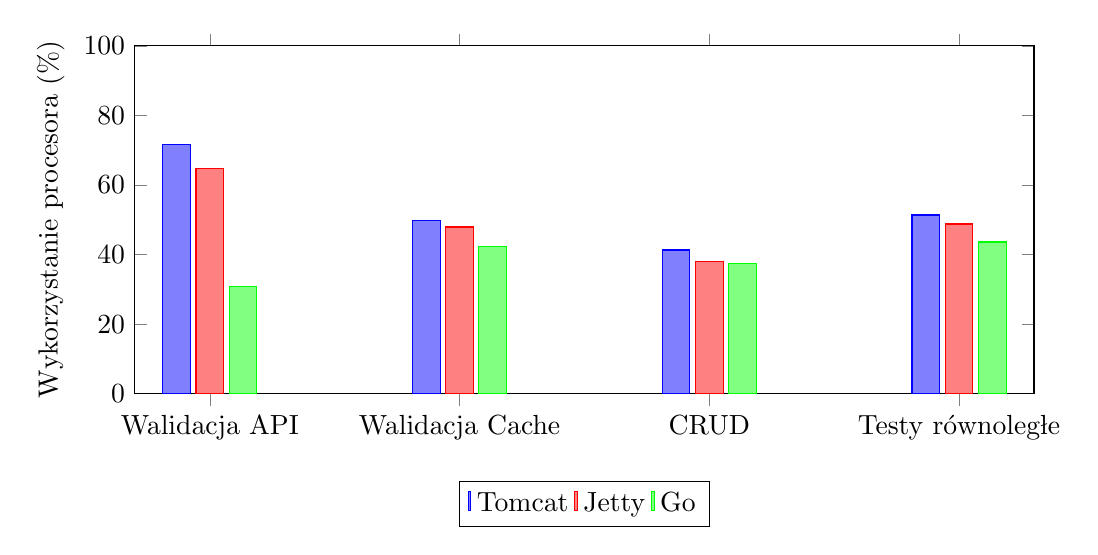
\begin{tikzpicture}
\begin{axis}[
    ybar,
    width=13cm,
    height=6cm,
    legend style={at={(0.5,-0.25)},
      anchor=north,legend columns=-1},
    ylabel={Wykorzystanie procesora (\%)},
     symbolic x coords={Walidacja API, Walidacja Cache, CRUD, Testy równoległe},
    xtick=data,
    ymin=0, ymax=100
    ]
\addplot [blue, fill=blue!50!white] coordinates{ (Walidacja API,71.62) (Walidacja Cache,49.82) (CRUD,41.32) (Testy równoległe,51.37) } ;
\addplot [red, fill=red!50!white] coordinates{ (Walidacja API,64.72) (Walidacja Cache,47.93) (CRUD,37.96) (Testy równoległe,48.79) } ;
\addplot [green, fill=green!50!white] coordinates{ (Walidacja API,30.79) (Walidacja Cache,42.43) (CRUD,37.34) (Testy równoległe,43.62) } ;
\legend{Tomcat,Jetty,Go}
\end{axis}
\end{tikzpicture}
\caption{Wykorzystanie procesowa przez aplikacje podczas testów z pustą bazą danych}
\label{fig:cpu_utilization_clean}
\end{figure}


\begin{figure}[!ht]
\begin{tikzpicture}
\begin{axis}[
    ybar,
    width=13cm,
    height=6cm,
    legend style={at={(0.5,-0.25)},
    anchor=north,legend columns=-1},
    ylabel={Wykorzystanie pamięci RAM (MB)},
    symbolic x coords={Walidacja API, Walidacja Cache, CRUD, Testy równoległe},
    xtick=data,
    ymin=0
]
\addplot [blue, fill=blue!50!white] coordinates{ (Walidacja API,1904.32) (Walidacja Cache,1972.46) (CRUD,1996.97) (Testy równoległe,2020.42) } ;
\addplot [red, fill=red!50!white] coordinates{ (Walidacja API,2012.54) (Walidacja Cache,1900.86) (CRUD,1679.41) (Testy równoległe,1772.25) } ;
\addplot [green, fill=green!50!white] coordinates{ (Walidacja API,220.19) (Walidacja Cache,224.31) (CRUD,232.18) (Testy równoległe,233.85) } ;
\legend{Tomcat,Jetty,Go}
\end{axis}
\end{tikzpicture}
\caption{Wykorzystanie pamięci na serwerze podczas testów z pustą bazą danych}
\label{fig:mem_utilization_clean}
\end{figure}


\begin{figure}[!ht]
\begin{tikzpicture}
\begin{axis}[
ybar,
width=13cm,
height=6cm,
legend style={at={(0.5,-0.25)},
anchor=north,legend columns=-1},
ylabel={Wykorzystanie procesora (\%)},
symbolic x coords={Walidacja API, Walidacja Cache, CRUD, Testy równoległe},
xtick=data,
ymin=0, ymax=100
]
\addplot [blue, fill=blue!50!white] coordinates{ (Walidacja API,60.97) (Walidacja Cache,42.12) (CRUD,27.96) (Testy równoległe,41.23) } ;
\addplot [red, fill=red!50!white] coordinates{ (Walidacja API,70.38) (Walidacja Cache,47.28) (CRUD,27.77) (Testy równoległe,35.66) } ;
\addplot [green, fill=green!50!white] coordinates{ (Walidacja API,31.87) (Walidacja Cache,32.27) (CRUD,23.57) (Testy równoległe,29.74) } ;
\legend{Tomcat,Jetty,Go}
\end{axis}
\end{tikzpicture}
\caption{Wykorzystanie procesowa na serwerze podczas testów z bazą danych wypełnioną danymi początkowymi}
\label{fig:cpu_utilization_full}
\end{figure}

\begin{figure}[!ht]
\begin{tikzpicture}
\begin{axis}[
ybar,
width=13cm,
height=6cm,
legend style={at={(0.5,-0.25)},
anchor=north,legend columns=-1},
ylabel={Wykorzystanie pamięci RAM (MB)},
symbolic x coords={Walidacja API, Walidacja Cache, CRUD, Testy równoległe},
xtick=data,
ymin=0
]
\addplot [blue, fill=blue!50!white] coordinates{ (Walidacja API,1948.69) (Walidacja Cache,2018.4) (CRUD,1902.79) (Testy równoległe,1852.85) } ;
\addplot [red, fill=red!50!white] coordinates{ (Walidacja API,1985.77) (Walidacja Cache,2050.25) (CRUD,2016.22) (Testy równoległe,2005.91) } ;
\addplot [green, fill=green!50!white] coordinates{ (Walidacja API,245.44) (Walidacja Cache,248.03) (CRUD,256.16) (Testy równoległe,257.09) } ;
\legend{Tomcat,Jetty,Go}
\end{axis}
\end{tikzpicture}
\caption{Wykorzystanie pamięci na serwerze podczas testów z bazą danych wypełnioną danymi początkowymi}
\label{fig:mem_utilization_full}
\end{figure}
\clearpage

\newpage
\section{Podsumowanie wyników}
